\documentclass{article}
\usepackage{graphicx}
\usepackage[utf8]{inputenc}
\usepackage[T1]{fontenc}
\usepackage{fouriernc}
\usepackage[margin=1in]{geometry}
\usepackage{amsmath}
\begin{document}

\begin{titlepage}
	\centering 
	\scshape
	\vspace*{\baselineskip}
	\rule{\textwidth}{1.6pt}\vspace*{-\baselineskip}\vspace*{2pt}
	\rule{\textwidth}{0.4pt} 
	\vspace{0.75\baselineskip}
	
	{\Large CS 374 : Computational and Numerical Methods \\\vspace{0.75\baselineskip} Set 17}
	\vspace{0.75\baselineskip}
	
	\rule{\textwidth}{0.4pt}\vspace*{-\baselineskip}\vspace{3.2pt} 
	\rule{\textwidth}{1.6pt}
	
	\vspace{2\baselineskip}  
	Systems of Differential Equations
	
	\vspace*{1\baselineskip}
	Prey-Predator Model
	
	\vspace{5\baselineskip} %originally 0.5
	
	{\scshape\large Purvil Mehta (201701073) \\ Bhargey Mehta (201701074) \\} 
	
	\vspace{1\baselineskip} 
	
	\textit{Dhirubhai Ambani Institute of Information and Communication Technology \\ Gandhinagar\\} 
	\vspace*{2\baselineskip}
	\today


\end{titlepage}

\tableofcontents

\newpage

\section{$y1 = 3, y2 = 5$}
\begin{figure}[!h]
    \centering
    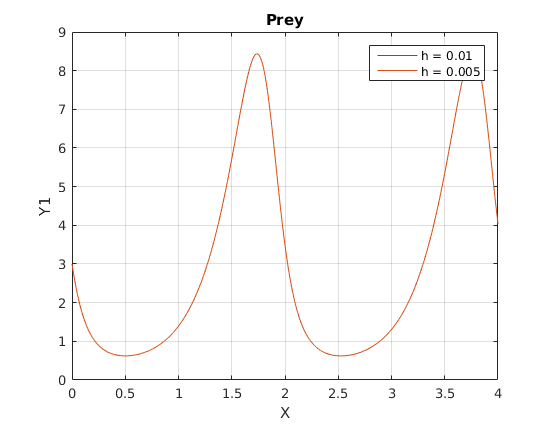
\includegraphics[scale = 0.6]{17_1.png}
    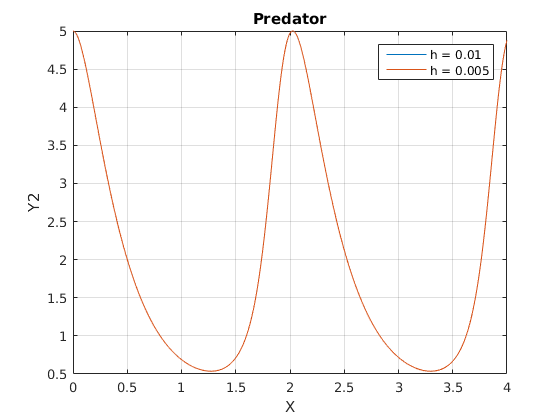
\includegraphics[scale = 0.6]{17_2.png}
    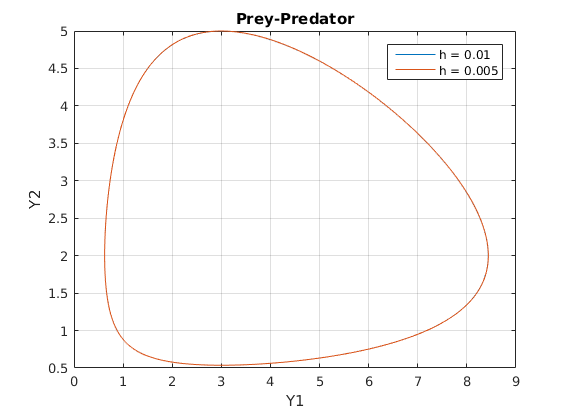
\includegraphics[scale = 0.6]{17_3.png}
    \caption{$y1 = 3, y2 = 5$}
\end{figure}

\section{$y1 = 3, y2 = 1$}
\begin{figure}[!h]
    \centering
    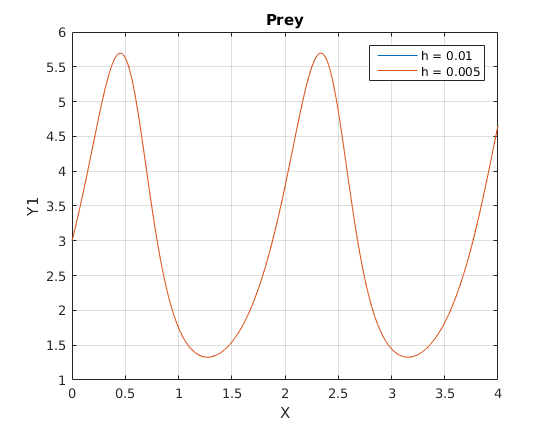
\includegraphics[scale = 0.6]{17_4.png}
    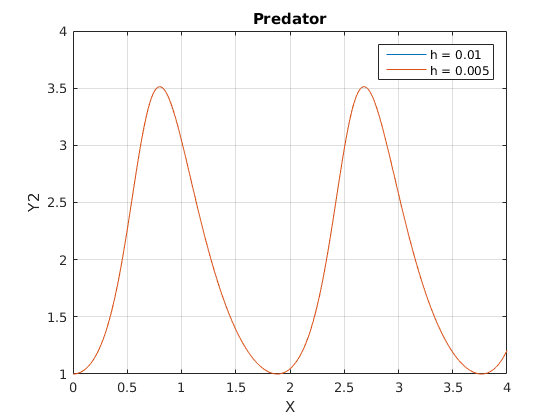
\includegraphics[scale = 0.6]{17_5.png}
    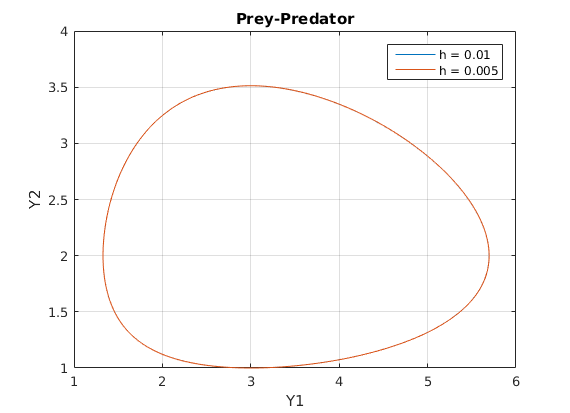
\includegraphics[scale = 0.6]{17_6.png}
    \caption{$y1 = 3, y2 = 1$}
\end{figure}

\section{$y1 = 3, y2 = 1.5$}
\begin{figure}[!h]
    \centering
    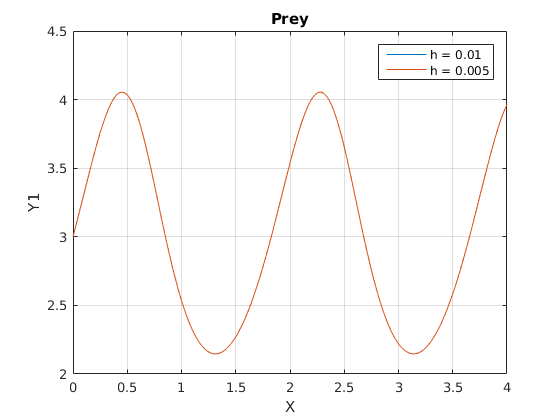
\includegraphics[scale = 0.6]{17_7.png}
    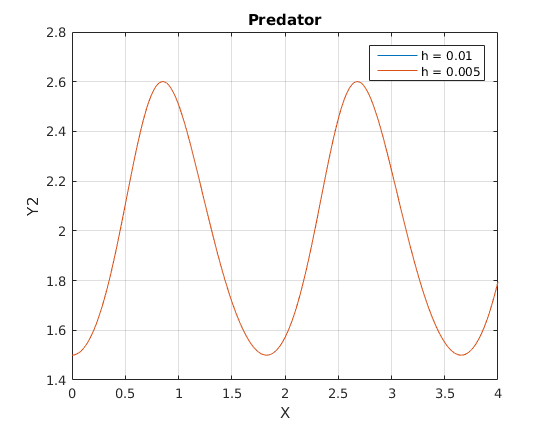
\includegraphics[scale = 0.6]{17_8.png}
    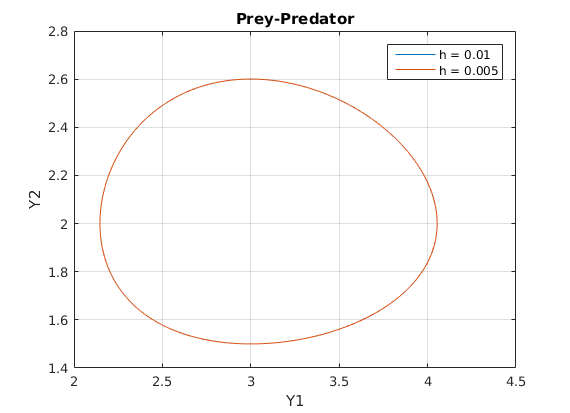
\includegraphics[scale = 0.6]{17_9.png}
    \caption{$y1 = 3, y2 = 1.5$}
\end{figure}

\section{$y1 = 3, y2 = 1.9$}
\begin{figure}[!h]
    \centering
    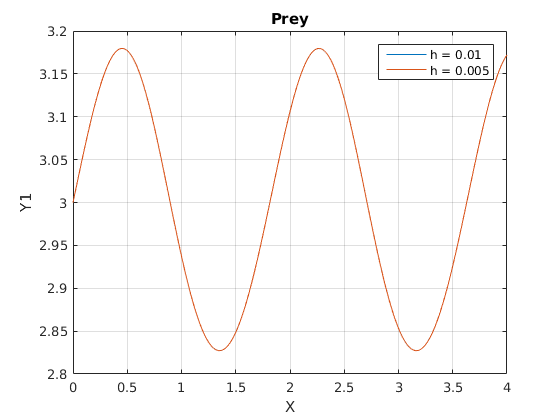
\includegraphics[scale = 0.6]{17_10.png}
    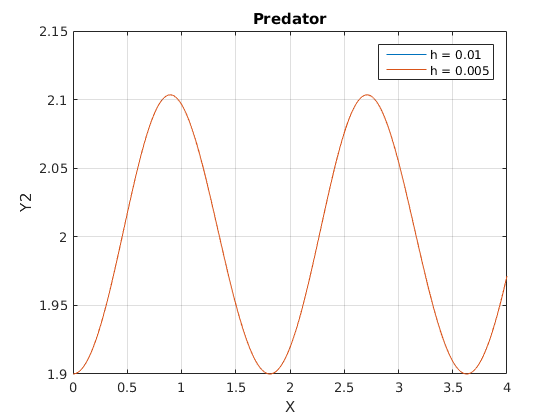
\includegraphics[scale = 0.6]{17_11.png}
    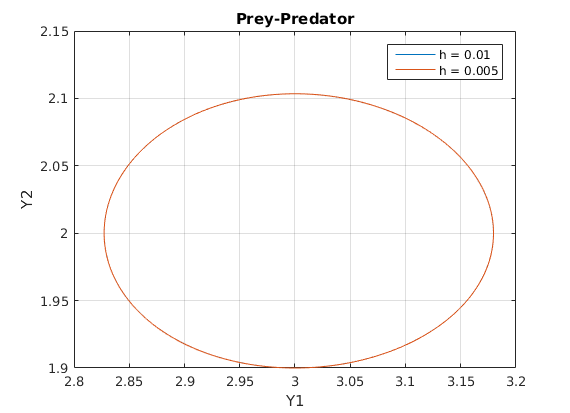
\includegraphics[scale = 0.6]{17_12.png}
    \caption{$y1 = 3, y2 = 1.9$}
\end{figure}
\end{document}